\documentclass[11pt,a4paper]{scrartcl}

% ------------------------- packages ------------------------------------------
% encoding and language
\usepackage[utf8]{inputenc}
\usepackage[ngerman, english]{babel}

% font
\usepackage[T1]{fontenc}
\usepackage{lmodern}

% hyperlink (URL, etc.)
\usepackage{hyperref}
%\usepackage{cleveref}

% citation
\usepackage{cite}

% math
\usepackage{amsmath}
\usepackage{amssymb}
\usepackage{nicefrac}

% code
\usepackage{listings}

% pseudocode
% \usepackage{algorithm}
% \usepackage{algpseudocode}
% \usepackage{algorithmicx}

% graphics
\usepackage{graphicx}
\usepackage{tikz}                 % includes xcolor
%\usetikzlibrary{arrows}
%\usetikzlibrary{shapes}

\newcommand{\diff}{\mathrm{d}}

\title{On the Stokes Jumps When Crossing the Singularity in the Borel Plane}
\date{\today}
\author{Marco Knipfer, \\ University of Alabama}
\begin{document}
\maketitle
Last lecture we had the question why ``crossing'' the singularity line $\theta$ in the Borel plane $\zeta$
results in a Stokes jump in the $x$-plane.

\section{Setup}
Remember the basic definitions of the Borel transform and Laplace transform (inverse Borel transform):
\begin{align}
	\tilde{\phi}(x) &\sim \sum_{n=0}^\infty \frac{a_n}{x^{n+1}}\,, \quad x\to \infty \,,&\text{asymptotic series} \\
	\hat{\phi}(\zeta) &\equiv \mathcal{B}[\tilde{\phi}](\zeta) = \sum_{n=0}^\infty \frac{a_n}{n!} \zeta^n\,,
			  &\text{Borel Transform}\\
	\mathcal{L}^\theta [\hat{\phi}](x) &= \int_0^{\infty e^{i \theta}}\diff\zeta\, \hat{\phi}(\zeta) e^{- \zeta x}\,,
					       &\text{Lateral Laplace Transform}\\
	S^\theta[\tilde{\phi}](x) &\equiv \mathcal{L}^\theta[\mathcal{B}[\tilde{\phi}]](x)\,, &\text{Lateral Borel Resummation}
\end{align}

Let's say we have an asymptotic series whose Borel transform has a simple pole\footnote{simple poles
are rather boring because they don't introduce a new instanton sector, we will adress this later} on the positive
real axis at $\zeta = A$.
We can either take $\theta = 0^-$ or $\theta = 0^+$ to do the Laplace transform, see figure~\ref{fig:laplaceContours}.
\begin{figure}
	\centering
	  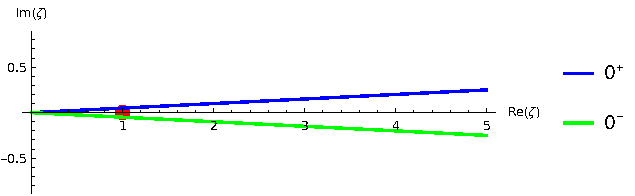
\includegraphics[width=0.8\linewidth]{laplace.pdf}
	  \caption{Contours of the different Laplace integrals.}
	  \label{fig:laplaceContours}
\end{figure}
The difference between both is simply
\begin{equation}
	\left( S^{0^-} - S^{0^+} \right)[\tilde{\phi}](x) = \underset{\zeta\to A}{\mathrm{Res}}(\hat\phi) e^{- A x}
	= k e^{-Ax}\,,
	\label{eq:ambiguity}
\end{equation}
which is nonanalytic in $x$ at our expansion point $x\to\infty$ and we have called the residue simply $k$.
Note that if the singularity was not only a simple pole, but a branch cut, then the difference would be a
whole new asymptotic series.

Another way of looking at the above structure is that we have a perturbative sector $\tilde\phi$ (= instanton action 0)
and an instanton sector $\phi_1$ which is just a constant.
Now, the general solution would consist of a linear combiantion of the perturbative series and the
instanton sector,
\begin{equation}
	Z(x) \sim \sigma_0 \tilde\phi(x) + \sigma_1 k e^{-Ax}\,.
\end{equation}

The ``instanton counting parameters'' $\sigma_0$ and $\sigma_1$ are determined by boundary conditions or other
considerations.

\section{Rotating in the $x$-Plane}
Say our boundary conditions have fixed $\sigma_0$ and $\sigma_1$ in the bottom right quadrant
$\Re(x)>0$,$\Im(x)<0$, then the resummed expansion in this region has the form
\begin{equation}
	Z_-(e^{-i\epsilon}x) \sim \sigma_0 S_{0^-}[\tilde\phi](e^{-i\epsilon}x) + \sigma_1 k e^{-A e^{-i\epsilon}x}\,,
		\quad x\in\mathbb{R}\to \infty
\end{equation}
where by $x e^{-i\epsilon}$ we make clear that we are talking about just below the real axis.
The Laplace transform in $S_{0^-}[\tilde\phi](x e^{-i\epsilon})$ then looks like
\begin{equation}
	\mathcal{L}^{0^-} [\hat{\phi}](x e^{-i\epsilon}) = \int_0^{\infty e^{-i \delta}}\diff \zeta\, \hat{\phi}(\zeta) e^{- \zeta x e^{-i\epsilon}}\,.
\end{equation}
Now let's see what happens if we go to just above the positive real axis in the $x$-plane:
\begin{align}
	\mathcal{L}^{0^-} [\hat{\phi}](x e^{+i\epsilon}) &= \int_0^{\infty e^{-i \delta}}\diff \zeta\, \hat{\phi}(\zeta) e^{- \zeta x e^{+i\epsilon}}\,.\\
	~&= \int_0^{\infty e^{-i (\delta-2\epsilon)}}\diff \xi e^{+ 2 i \epsilon}\, \hat{\phi}(\xi e^{2 i \epsilon}) e^{- \xi x e^{-i\epsilon}}\,,
	\intertext{and upon chosing $\delta = \epsilon$,}
	~&= e^{+ 2 i \epsilon}\int_0^{\infty e^{+ i\epsilon}}\diff \xi \, \hat{\phi}(\xi e^{2 i \epsilon}) e^{+ \xi x e^{-i\epsilon}}\,.
	\intertext{
We see that now we are integrating along $\theta = 0^+$ and also in $\hat\phi(\xi e^{2 i \epsilon})$ the singularity has
been shifted to below the real axis, so as I physicists I would say this is in the limit $\epsilon \to 0^+$}
	~&= \mathcal{L}^{0^+}[\hat\phi](x e^{-i\epsilon})\,.
\end{align}
In other words: If we take the same resummation definition (the contour) and simply vary $x$ from just below the
real axis to just above the real axis, then this is the same as just changing the contour from just below the singularity
to just above the singularity.
Thus when crossing the Stokes line $(0,\infty)$ in $x$ we effectively go from $S^{0^-}$ to $S^{0^+}$ and the difference
is
\begin{equation}
	k e^{-A x}\,.
\end{equation}
Thus in the transseries
\begin{align}
	&Z(e^{-i\epsilon}x, \sigma_0, \sigma_1) \sim \sigma_0 \tilde\phi(x) + \sigma_1 e^{-Ax}\,.
	\intertext{we add the term (\ref{eq:ambiguity})}
	&Z(e^{+i\epsilon}x, \sigma_0, \sigma_1) \sim \sigma_0 \tilde\phi(x) + (\sigma_1 + k) e^{-Ax}\,.
\end{align}
We have arived at the formula
\begin{equation}
Z(e^{+i\epsilon}x, \sigma_0, \sigma_1)  = Z(e^{-i\epsilon}x, \sigma_0, \sigma_1 + k)
\end{equation}

\section{Details that are not clear to me yet}
I am not sure about $\delta$ and $\epsilon$ in above argument.
Probably one has to chose them the same per definition, but maybe there is some more structure that
I am not seing right now.

\end{document}
